\subsection{紧空间的正则性}

命题 I. 设 X 是紧空间，x 是 X 的一点。为使由 x 的闭邻域组成的一个滤子基 B 是 x 的基本邻域系，必要且充分的是 B 中诸集合之交仅由 x 组成。

该条件是必要的，因为 X 是豪斯多夫的（§ 8，第 1 目，命题 1）。它也是充分的，因为它意味着 x 是 B 的唯一聚点；于是由第 1 目定理 1 的推论，B 收敛于 x。

推论. 每个紧空间都是正则的。

因为由公理 (Hi)（§ 8，第 1 目，命题 1），由该空间任一点的所有闭邻域组成的滤子基满足命题 I 的条件。

下面的命题加强了命题 I 的推论：

命题 2. 设 X 是紧空间，并设 A, B 是 X 的两个不相交的闭子集。则存在两个开集 U, V，使得 \(U \cap V = \varnothing\) 且 \(A \subset U\) 且 \(B \subset V\)。

设结论不真。若 A 的每个邻域 U 都与 B 的每个邻域 V 相交，则诸集合 \(U \cap V\) 在 X 上构成一个滤子基 B，从而它有一个聚点 \(x \in X\)。现在 x 必属于 A，因为若 y 是 X 中不属于 A 的任一点，则由于 X 是正则的，存在 y 的一个邻域与 A 的一个邻域，二者不相交，从而 y 不可能是 B 的聚点。类似地，x 必属于 B，于是得到矛盾。

\pandocbounded{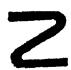
\includegraphics[keepaspectratio]{images/part001_de955d1b.jpg}}

这个命题有重要的推论，将在第九章 § 4 中考察。

第 1 目例 2 中的非豪斯多夫拟紧空间 X 既不满足公理 (O \(_{III}\) )，更不满足命题 2 所述的性质，因为这个空间的任意两个非空开集总相交。

